\subsection{Implementierung} \label{sec:implementierung}
Die Implementierung richtet sich in wesentlichen Zügen an der Ausarbeitung des dritten Kapitels des eingangs erwähnten Buches \cite{buch}. Im Folgenden werden die wichtigsten Punkte zusammengefasst. Das \ac{dg}-Verfahren wird dabei der Einfachheit halber zunächst als eindimensional angesehen mit $v\fin \in X_{\mathcal{T},1}$. An relevanten Stellen wird die Einbettung in das System mit $v\fin \in X\fin$ berücksichtigt, vergleiche Gleichung \eqref{eq:FES}.

Die Ritz-Approximation $v\fin \in X_{\mathcal{T},1}$ ist lokal definiert. \emph{Lokal}\index{lokale Darstellung der Ritz-Approximation} bedeutet hier stets eine elementweise Betrachtung für jedes Element $D^k$. Wie in jedem \ac{fem}-Verfahren überführt die affine Abbildung
\begin{equation}
  x\in D^k : \qquad x(r) = x_{k-\nicefrac{1}{2}} + \frac{1+r}{2}h_k, \qquad h_k=x_{k+\nicefrac{1}{2}} - x_{k-\nicefrac{1}{2}}
  \label{eq:affmap}
\end{equation}
die lokalen Integrale auf ein Referenzelement $I=[-1,1]$ mit $r\in I$.
Es wird dann zwischen \emph{modaler Darstellung}\index{modale Darstellung}
\begin{align}
  x\in D^k : \qquad v\fin^k(r(x),t) = \sum_{n=1}^{N_p}\hat{v}_{\mathcal{T},n}^k(t) \Phi_n(r)
\end{align}
und \emph{nodaler Darstellung}\index{nodale Darstellung}
\begin{align}
  x\in D^k : \qquad v\fin^k(r(x),t) = \sum_{i=1}^{N_p} v_{\mathcal{T},i}^k(t)\ell_i(r)
  \label{eq:nodal}
\end{align}
der Ritz-Approximation unterschieden. Dabei sind $\Phi_n(r)$ bzw. $\ell_i(r)$ verschiedene Basisfunktionen des Polynomraumes $P_N(I)$ (siehe auch Gleichung \eqref{eq:FES}). Für das System hat $v\fin^k(x,t)$ gerade $K_y$ Komponenten. Die entsprechenden Koeffizienten bekommen dann einen weiteren Index $v_{\mathcal{T},i}^k \rightarrow v_{\mathcal{T},i}^{k,j}$ mit $j=1,\dots,K_y$.

Die nodale Darstellung bietet den Vorteil, dass die Funktion nicht unbedingt ausgewertet werden muss, da $v\fin^k(x(\xi_i),t)$ durch die Entwicklungskoeffizienten $v_{\mathcal{T},i}^k(t)$ bereits gegeben ist. Es handelt sich hierbei also um eine interpolatorische Darstellung.
Eine hierfür geeignete Basis sind die Lagrange-Polynome
\begin{align}
  \ell_i(r) = \prod_{\substack{j=1 \\ j\neq i}}^{N_p} \frac{r-\xi_j}{\xi_i-\xi_j}
  \label{eq:nodalebasis}
\end{align}
mit $N_p$ verschiedenen Knotenpunkten $\xi_j\in[-1,1]$ und der Eigenschaft ${\ell_i(\xi_j)=\delta_{ij}}$. Für eine Verallgemeinerung in höherdimensionale Probleme bietet es sich an, die benötigten Integrale über die Basisfunktionen mit Hilfe der modalen Basis $\Phi$ zu kalkulieren, da die Lagrange-Polynome sich nicht auf einfache Weise formulieren lassen. Für diese modale Basis wird für eine gute Konditionierung der Massenmatrix (vergleiche Gleichung \eqref{eq:Mmatrix}) statt der Monombasis die orthonormierte Basis
\begin{align}
  \Phi_n(r) = \frac{P_{n-1}(r)}{\sqrt{2(2n+1)^{-1}}}
  \label{eq:modaleBasis}
\end{align}
mit den Legendre Polynomen $P_n(r)$ gewählt. Der Zusammenhang zwischen nodaler und modaler Basis ist durch die \emph{Vandermonde-Matrix}\index{Vandermonde-Matrix}
\begin{equation}
  \begin{aligned}
    \van_{ij} = \Phi_j(\xi_i)
  \end{aligned}
  \label{eq:vandermonde}
\end{equation}
gegeben. Es gilt dann
  \begin{align}
    &\van\hat{v}\fin = v\fin        & &\text{sowie} \label{eq:nodalmodal}\\
    &\van^T\ell(r) = \Phi(r) & &\text{mit} \label{eq:ellPsi}\\
    &\hat{v}\fin = (\hat{v}_{\mathcal{T},1} \dots \hat{v}_{\mathcal{T},N_p})^T, & & v =(v_{\mathcal{T},1} \dots v_{\mathcal{T},N_p})^T \nonumber \\
    &\ell(r) = (\ell_1(r) \dots \ell_{N_p}(r))^T, & & \Phi(r) =(\Phi_1(r) \dots \Phi_{N_p}(r))^T \nonumber \; ,
  \end{align}
wobei der Index $\mathcal{T}$ der Übersicht halber temporär unterdrückt worden ist. Der Zusammenhang gilt wegen der affinen Abbildung \eqref{eq:affmap} für alle Elemente $D^k$, weshalb auch dieser Index unterdrückt worden ist.

Die Interpolationspunkte $\xi_j$ werden derart gewählt, dass die Interpolation möglichst nahe an der bestmöglichen Ritz-Approximation durch ein (allgemeines) Polynom liegt. Dies führt auf die Legendre-Gauß-Lobatto Quadraturpunkte. Besonders für hohe Polynomgrade $N\geq 5$ ist diese Wahl zu favorisieren, denn äquidistante Knoten würden hier zu einer exponentiell schlecht konditionierten Interpolation führen. Ein weiterer Vorteil offenbart sich, wenn für die spätere Fehlerberechnung die Funktion über $\Omega$ integriert werden muss. Hier bietet sich dann die Gauß-Lobatto-Quadratur an, sodass die Funktionsauswertung nach Gleichung \eqref{eq:nodal} entfällt, da lediglich $v\fin(\xi_j)$ benötigt wird und diese Funktionswerte gerade den Koeffizienten entsprechen.

Mit diesen Vorarbeiten kann nun die starke Formulierung \ref{prob:strong} in eine Matrix-Vektor-Gleichung überführt werden. Die Forderung der Gültigkeit für alle Testfunktionen $\varphi\in X_{\mathcal{T},1}$ übersetzt sich für einen $N_p$-dimensionalen Polynomraum in exakt $N_p \times K_x$ Gleichungen. Für das gesamte System mit $K_y$ Zellen in $y$-Richtung müssen sich entsprechend $N_p \times K_x \times K_y$ Gleichungen ergeben. Dazu wird lokal als Testfunktion $\varphi = \ell_m e_j$ gewählt mit dem Einheitsvektor $e_j$, wobei $m=1\dots N_p$ und $j=1\dots K_y$. Für die weitere Notation sowie die Implementierung dient die folgende Definition.
\begin{definition}[Massen- und Steifigkeits- und Driftmatrix, Notation der Lösung]\index{Massematrix}\index{Steifigkeitsmatrix}\index{Driftmatrix} \label{def:matrizen}
  Für die nodale Darstellung heißen
  \begin{equation*}
    (M^k)_{pq} \equiv \int_{x_{k-\nicefrac{1}{2}}}^{x_{k+\nicefrac{1}{2}}} \ell_p^k(x) \ell_q^k(x) \diff x = \frac{h_k}{2}\int_{-1}^1 \ell_p(r) \ell_q(r) \diff r \equiv \frac{h_k}{2} M_{pq}
    \label{eq:Mmatrix}
  \end{equation*}
  Massenmatrix,
  \begin{equation*}
    (S^k)_{pq} \equiv \int_{x_{k-\nicefrac{1}{2}}}^{x_{k+\nicefrac{1}{2}}} \ell_p^k(x) \td{\ell_q^k(x)}{x} \diff x = \int_{-1}^1 \ell_p(r) \td{\ell_q(r)}{r}  \diff r \equiv S_{pq}
    \label{eq:Smatrix}
  \end{equation*}
  Steifigkeitsmatrix und
  \begin{equation*}
    (\drift^{k,jm})_{pq} = \int_{D^k} G_{jm}(x) \ell_p^k(x) \ell_q^k(x) \diff x \qquad \forall j,m=1\dots K_y % v_{\mathcal{T},p}^{k,m} wird dadran multipliziert
  \end{equation*}
  Driftmatrix. Dabei ist $G_{jm}(x)$ die Matrixkomponente von $G(x)$ aus Gleichung \eqref{eq:G}. Hier und im Folgenden ist die explizite Zeitabhängigkeit temporär unterdrückt worden. Die nodalen Entwicklungskoeffizienten der Lösung des Variationsproblems $v\fin$ werden gemäß
  \begin{equation*}
    \begin{aligned}
      \underline{v} &= (\underline{v}_1 \dots \underline{v}_{K_y})^T        &  &\text{mit} \\
      \underline{v}_j &= (\underline{v}_j^1 \dots \underline{v}_j^{K_x})^T  &  &\text{mit} \\
      \underline{v}_j^k &= (v_{\mathcal{T},1}^{k,j} \dots v_{\mathcal{T},N_p}^{k,j})^T
    \end{aligned}
  \end{equation*}
  notiert und somit in einem globalen Vektor $\underline{v} \in \mathbb{C}^{s}$ mit $s=K_y K_x N_p$ zusammengefasst.
\end{definition}
Genau wie die bereits für das System definierte Driftmatrix lassen sich auch $M$ und $S$ für das System definieren. Sie sind bezüglich der $y$-Richtung blockdiagonal gemäß $(\mathcal{M}^{k,jm})_{pq} = \delta_{jm}(M^k)_{pq}$ und $\mathcal{S}$ analog.
Die eingeführten Matrizen lassen sich durch die Vandermondematrix $\van$ ausdrücken. Die Zusammenhänge für Massen- und Steifigkeitsmatrix sind durch
\begin{align*}
  M &= (\van\van^T)^{-1} \\
  M^{-1}S &= \van_r \van^{-1} \qquad \text{mit } (\van_r)_{ij} = \td{\Phi_j}{r}\biggr\rvert_{\xi_i}
\end{align*}
gegeben, wobei im Wesentlichen die Orthonormiertheit der gewählten modalen Basis \eqref{eq:modaleBasis} eingegangen ist. Für die Driftmatrix wird im Anhang \ref{sec:A_5} ein entsprechender Ausdruck hergeleitet. Es ist hierzu anzumerken, dass die Driftmatrix die einzige Kopplung bezüglich $y$-Richtung darstellt. Daher geht die Herleitung über eine eindimensionale Betrachtung des \ac{dg}-Verfahrens und damit über die Ausführungen in \cite{buch} hinaus.

Prinzipiell gibt es verschiedene Möglichkeiten, den Driftterm zu behandeln. Da jedoch Funktionswerte Von Ansatz- und Testfunktion bereits an den Gauß-Lobatto Quadraturpunkten vorliegen, bietet es sich an, diese Quadratur zu verwenden. Es wird im folgenden zwischen zwei Methoden unterschieden.
\begin{enumerate}
  \item (Methode G1) Es lässt sich von vornherein das Produkt $G(x)v\fin(x)$ in der nodalen Basis entwickeln. Dann ergibt sich für das resultierende Integral wieder die Massenmatrix. In dem lokalen Schema verbleibt dann nach Multiplikation mit $(M^k)^{-1}$ schlicht der Ausdruck ${\sum_{m=1}^{K_y}\text{diag}(\underline{G}^k_{jm})\underline{v}_m^k}$. Die Driftmatrix aus Definition \ref{def:matrizen} findet hierbei nicht Verwendung.
  \item (Methode G2) Eine genauere Betrachtung belässt $G(x)$ als analytisch bekannt, sodass die Driftmatrix mit Hilfe von Gauß-Lobatto-Quadratur höherer Ordnung berechnet werden kann. Mit der Quadraturordnung $N_{GL}$ ergibt sich mit den dem Anhang \ref{sec:A_5} zu entnehmenden Definitionen der Matrix $W$ und der Gewichte $w$
  \begin{equation}
    (\drift^{k,jm})_{pq} = \sum_{a=1}^{N_{GL}} W_{ap} W_{ai} w_a G_{jm}(\xi_a^k)\frac{h_k}{2} \; .
    \label{eq:G_GL}
  \end{equation}
  Diese Methode ist insbesondere für unstetige Potentiale wie das Flachbandpotential in Abbildung \ref{fig:pot1} zu bevorzugen, da solche Unstetigkeiten besser durch Polynome höherer Ordnung approximiert werden.
\end{enumerate}
Beide Ansätze sind numerisch anhand der resultierenden iterativen Fehler verglichen worden, siehe Kapitel \todo{ref}. Es zeigt sich erwartungsgemäß, dass der zweite Ansatz zu besseren Konvergenzraten führt. Offensichtlich ist dies aber gleichzeitig die rechenintensivere Option.

Nun lässt sich das Variationsproblem \ref{prob:strong} zunächst für festen Index $j$ und innere Elemente lokal umschreiben gemäß
\begin{equation}
  \begin{aligned}
    \forall D^k\in\mathcal{T} \textbackslash &\{D^1,D^{K_x}\} : \\
      &\partial_t \underline{v}_j^k + (M^k)^{-1}S \underline{f}_j^k + \sum_{m=1}^{K_y} (M^k)^{-1}\drift^{k,jm}\underline{v}_m^k \\
      &+ \left(\frac{-\lambda_j + |\lambda_j|}{2}\right) \jump{\underline{v}_j}_{e_r}\underline{E_r} +
         \left(\frac{-\lambda_j - |\lambda_j|}{2}\right) \jump{\underline{v}_j}_{e_l}\underline{E_l} = 0
  \end{aligned}
  \label{eq:schema1}
\end{equation}
wobei die lokalen \emph{Liftoperatoren}\index{Liftoperator}
\begin{equation}
  \begin{aligned}
    \underline{E_r} &\equiv (M^k)^{-1}\underline{\ell}(x_{k+\nicefrac{1}{2}}) = (M^k)^{-1}  \cdot (0,\dots,0,1)^T \\
    \underline{E_l} &\equiv (M^k)^{-1}\underline{\ell}(x_{k-\nicefrac{1}{2}}) = (M^k)^{-1}  \cdot (1,0,\dots,0)^T
  \end{aligned}
\end{equation}
eingeführt worden sind. Die letzte Gleichheit ergibt sich für Polynomgrade $N\geq{1}$, da ${ \{x_{k-\nicefrac{1}{2}}, x_{k+\nicefrac{1}{2}}\} = \{\xi_1, \xi_{N^p} \} }$ für die gewählten Gauß-Lobatto Quadraturpunkte. Der Sprung der Koeffizienten ist etwas fahrlässig notiert, um die Situation nicht unnötig unleserlich zu gestalten. Es ist für innere Kanten
\begin{align*}
  \jump{\underline{v}_j}_{e_r} &= v_{\mathcal{T},N_p}^{k,j} - v_{\mathcal{T},1}^{k+1,j} \qquad \text{und} \\
  \jump{\underline{v}_j}_{e_l} &= v_{\mathcal{T},1}^{k,j} - v_{\mathcal{T},N_p}^{k-1,j}
\end{align*}
gesetzt worden gemäß der Definition \eqref{eq:jump_def_inner}. Dieser Ausdruck entspricht wegen der interpolatorischen Eigenschaft der Lagrange-Polynome exakt dem Sprung der Ritz-Approximation. Die Zusammenhänge werden in Abbildung \ref{fig:notationDG2} veranschaulicht.
\begin{figure}
  \centering
  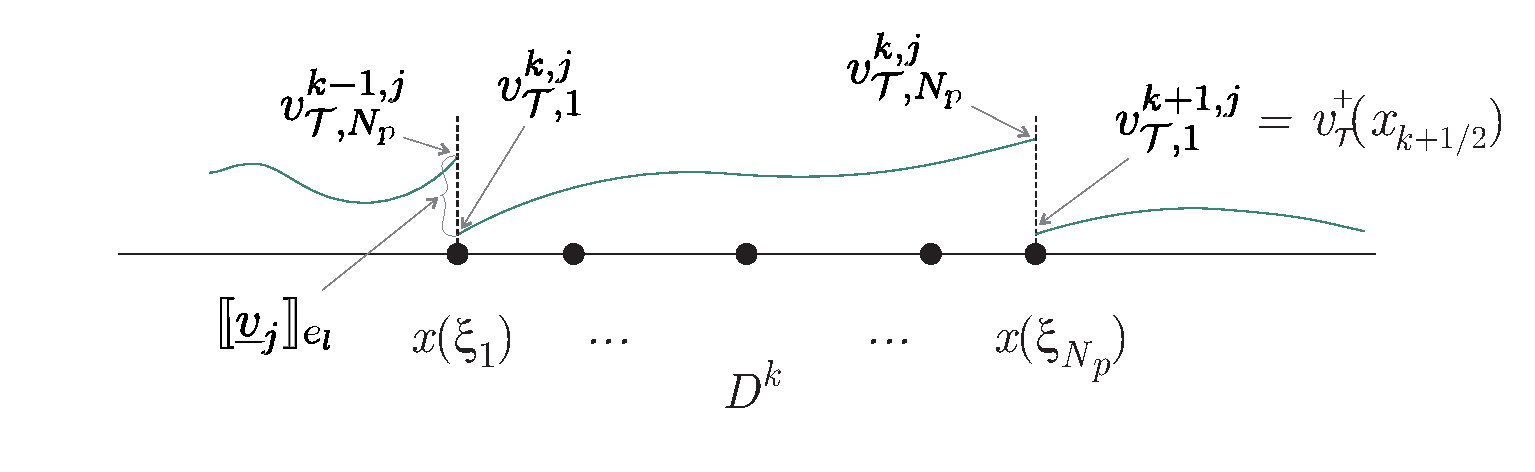
\includegraphics[width=0.95\textwidth]{files/notationDG2.pdf}
  \caption{Notation der nodalen Darstellung für das eindimensionale \ac{dg}-Verfahren. An den Knotenpunkten entspricht der Funktionswert gerade den Entwicklungskoeffizienten. Da für Gauß-Lobatto Knoten mit $N_p\geq 2$ stets $\xi_1=-1$ und $\xi_{N_p}=1$ gilt, entspricht der Sprung von $v\fin$ dem Sprung der Koeffizienten.}
  \label{fig:notationDG2}
\end{figure}
Für die beiden Randelemente ergibt sich
\begin{equation}
  \begin{aligned}
      &\partial_t \underline{v}_j^{K_x} + (M^{K_x})^{-1}S \underline{f}_j^{K_x} + \sum_{m=1}^{K_y} (M^{K_x})^{-1}\drift^{k,jm}\underline{v}_m^{K_x} \\
      &+ \left(\frac{-\lambda_j + |\lambda_j|}{2}\right) v_{\mathcal{T},N_p}^{K_x,j} \underline{E_r} +
         \left(\frac{-\lambda_j - |\lambda_j|}{2}\right) \jump{\underline{v}_j}_{e_l}\underline{E_l} =
         \left(\frac{-\lambda_j + |\lambda_j|}{2}\right) g_j(x_r,t)\underline{E_r}
  \end{aligned}
  \label{eq:schema2}
\end{equation}
\begin{equation}
  \begin{aligned}
      &\partial_t \underline{v}_j^{1} + (M^{1})^{-1}S \underline{f}_j^{1} + \sum_{m=1}^{K_y} (M^{1})^{-1}\drift^{k,jm}\underline{v}_m^{1} \\
        &+ \left(\frac{-\lambda_j + |\lambda_j|}{2}\right) \jump{\underline{v}_j}_{e_r}\underline{E_r} +
           \left(\frac{\lambda_j + |\lambda_j|}{2}\right) v_{\mathcal{T},1}^{1,j} \underline{E_l}
        =\left(\frac{\lambda_j + |\lambda_j|}{2}\right) g_j(x_l,t)\underline{E_l} \; .
  \end{aligned}
  \label{eq:schema3}
\end{equation}
Die Gleichungen \eqref{eq:schema1}, \eqref{eq:schema2}, \eqref{eq:schema3} werden in stationärer Form (das heißt $\partial_t \underline{v}=0$) als globales Matrix-Vektor-System implementiert, sodass das lineare Gleichungssystem
\begin{equation}
  \underline{\underline{\mathcal{A}}}\,\underline{v} = \underline{b}
  \label{eq:stat_LGS}
\end{equation}
resultiert mit der Systemmatrix $\underline{\underline{\mathcal{A}}}$ sowie dem Vektor $\underline{b}$, der sich aus der rechten Seite von \eqref{eq:schema2} bzw. \eqref{eq:schema3} ergibt und die Randbedingungen enthält. Zur Lösung des LGS wird die \mat-interne Methode verwendet. Die gesuchte stationäre Dichtematrix ergibt sich schließlich aus der Rücktransformation \eqref{eq:trafo_uv}. Für die Zeitentwicklung wird dann ein explizites Zeitschrittverfahren angewandt, siehe Abschnitt \ref{sec:timestepping}.

Die Bestandteile der Systemmatrix werden in den folgenden Abbildungen für die Systemgröße $\{K_x=3, N_p=3, K_y=4\}$ exemplarisch gezeigt. Sie unterteilt sich in den Diffusionsterm $(M^k)^{-1}S\Lambda$, den Driftterm $(M^k)^{-1}\mathcal{G}^k$ sowie den Flussterm, welcher die Kantenterme beinhaltet. Die Abbildungen sind zur Verbesserung der Lesbarkeit mit einer farblichen Struktur unterlegt. Dabei ist Definition \ref{def:matrizen} hilfreich. Die grünen Rahmen bedeuten fixierte $y$-Diskretisierung (Indizes $j,m$ konstant). Die grauen Quadrate beranden ein Element der $x$-Diskretisierung ($D^k$ konstant), worin wiederum die $N_p \times N_p$ lokal definierten Matrizen $M^k$, $S^k$ und $\mathcal{G}^{k,jm}$ zu sehen sind.

Abbildung \ref{fig:matrix_L} zeigt den Diffusionsterm.
\begin{figure*}
    \centering
    \begin{subfigure}[b]{0.475\textwidth}
        \centering
        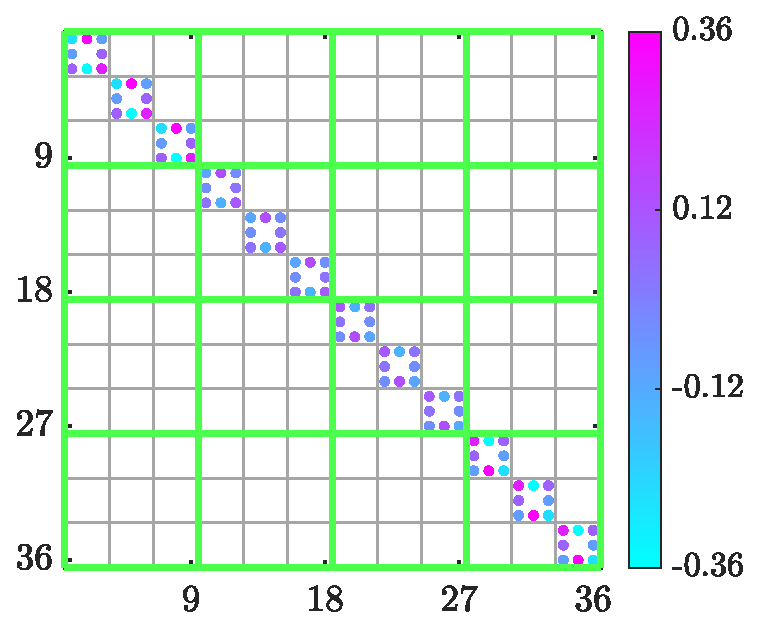
\includegraphics[width=\textwidth]{plots/L_glob.eps}
        \caption[]%
        {{\small Diffusionsmatrix}}
        \label{fig:matrix_L}
    \end{subfigure}
    \hfill
    \begin{subfigure}[b]{0.475\textwidth}
        \centering
        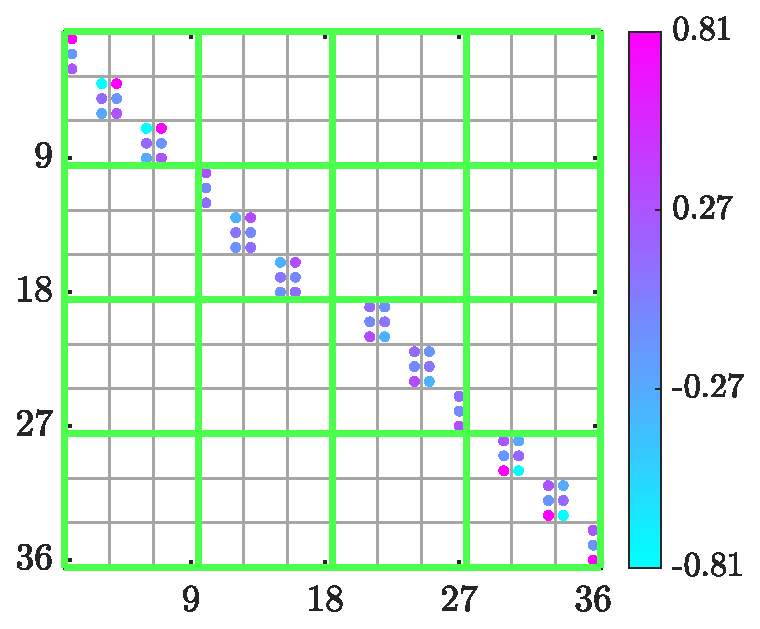
\includegraphics[width=\textwidth]{plots/F_glob.eps}
        \caption[]%
        {{\small Flussmatrix}}
        \label{fig:matrix_F}
    \end{subfigure}
    \caption[]
    {Struktur der beiden Flussmatrizen in willkürlichen Einheiten. Links sind die Volumenteile und rechts die ursprünglich aus der partiellen Integration entstammenden Kantenbeiträge abgebildet. In der Flussmatrix enthalten ist der numerische Fluss. Dieser bringt die einzigen Nebendiagonalbeiträge der Systemmatrix in $x$-Richtung ein und stellt somit die Kopplung zwischen Zellen dar.}
    % \label{fig:Schaltungen}
\end{figure*}
Wegen der um 0 symmetrisch verteilten Eigenwerte \eqref{eq:Lambda} ist diese Matrix rotations- oder doppelt spiegelsymmetrisch. Auch tendieren deshalb die nominellen Werte von außen Richtung Mitte der Matrix gegen 0. Innerhalb eines grün umrandeten Blocks entstehen bei äquidistanter Diskretisierung  $K_x$ Replika. Die Matrix ist blockdiagonal, da der entsprechende Term in Gleichung \eqref{eq:diagLVN} bereits diagonal ist.

Eine ähnliche Struktur zeigt sich für die Flussmatrix in Abbildung \ref{fig:matrix_F}. Dieselbe Symmetrie ergibt sich aus denselben Gründen, jedoch finden sich in dieser Matrix die Kopplungen zwischen benachbarten Elementen wieder. Für die obere linke Hälfte ist $\lambda_j>0$, sodass der numerische Fluss als Upwind Fluss \index{Upwind Fluss} Werte aus der linksseitigen Nachbarzelle einbezieht. Unten rechts ist $\lambda_j<0$ und es werden rechtsseitige Nachbarzellen berücksichtigt. Am Rand (oben links bzw. unten rechts) "fehlen" Werte, welche in der rechten Seite als Randbedingung $b$ wiederzufinden sind.

Abbildung \ref{fig:matrix_G} zeigt die Driftmatrix für verschiedene Fälle.
\begin{figure*}
    \centering
    \begin{subfigure}[b]{0.488\textwidth}
        \centering
        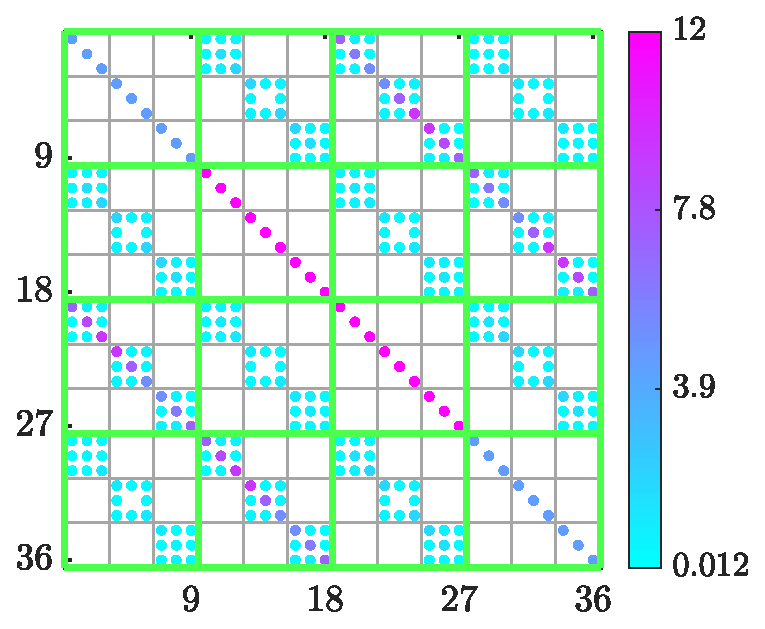
\includegraphics[width=\textwidth]{plots/absG_glob_w_GL_w_CAP.eps}
        \caption[]%
        {{\small $W_0<0$, Methode G2.}}
        \label{fig:G_1}
    \end{subfigure}
    \hfill
    \begin{subfigure}[b]{0.462\textwidth}
        \centering
        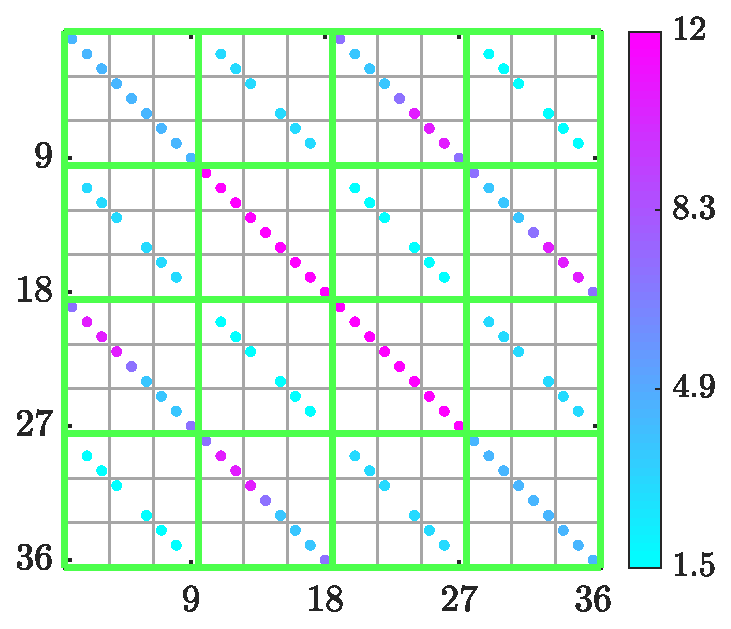
\includegraphics[width=\textwidth]{plots/absG_glob_wo_GL_w_CAP.eps}
        \caption[]%
        {{\small $W_0<0$, Methode G1.}}
        \label{fig:G_2}
    \end{subfigure}
    \vskip\baselineskip
    \begin{subfigure}[b]{0.488\textwidth}
        \centering
        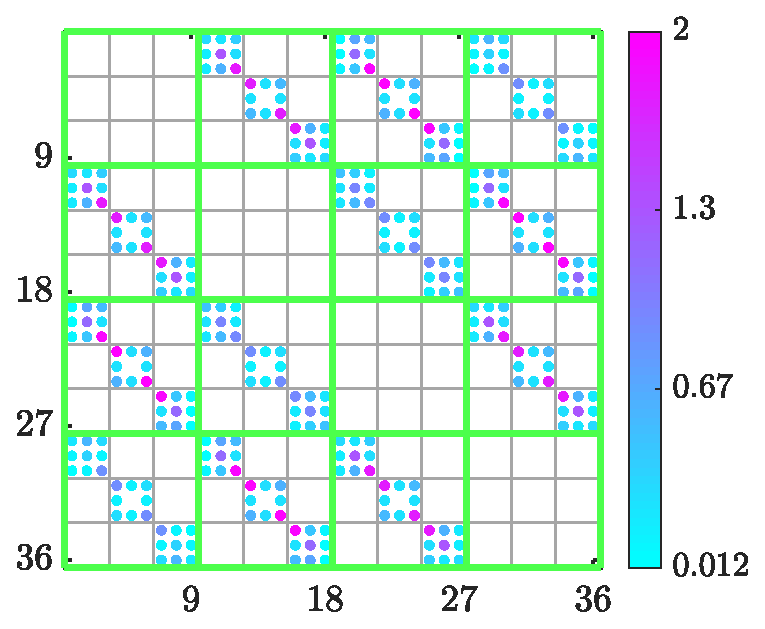
\includegraphics[width=\textwidth]{plots/absG_glob_w_GL_wo_CAP.eps}
        \caption[]%
        {{\small $W_0=0$, Methode G2.}}
        \label{fig:G_3}
    \end{subfigure}
    \quad
    \begin{subfigure}[b]{0.462\textwidth}
        \centering
        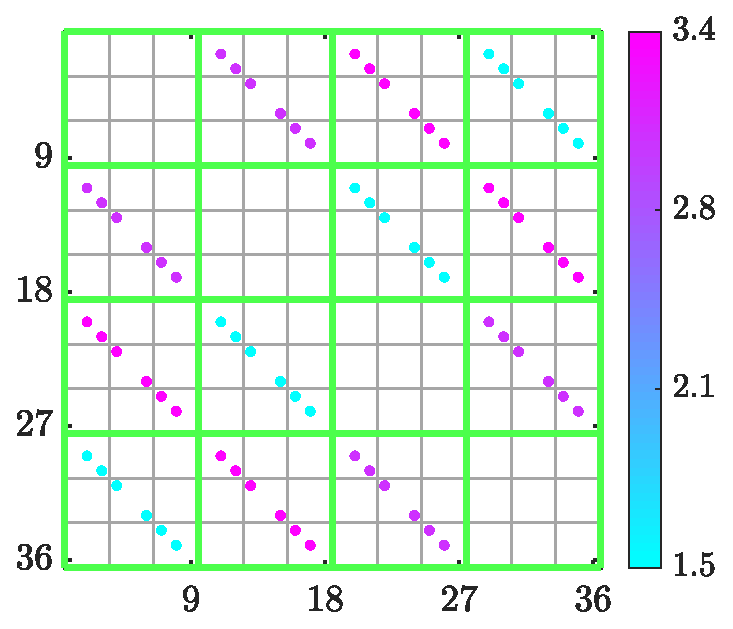
\includegraphics[width=\textwidth]{plots/absG_glob_wo_GL_wo_CAP.eps}
        \caption[]%
        {{\small $W_0=0$, Methode G1.}}
        \label{fig:G_4}
    \end{subfigure}
    \caption[]
    {Betrag der Driftmatrix für verschiedene Fälle in willkürlichen Einheiten. Die beiden linken Teile sind mit Gauß-Lobatto Quadratur berechnet, rechtsseitig ist das Produkt $G(x)v\fin(x)$ in der nodalen Basis entwickelt worden (siehe oben). Für die beiden oberen Teile ist das \ac{cap} eingeschaltet (vgl. \eqref{eq:cap}), unten ist es ausgeschaltet.}
    \label{fig:matrix_G}
\end{figure*}
Zunächst ist hierzu anzumerken, dass die Matrix den einzig komplexen Beitrag zur Systemmatrix liefert -- gezeigt ist an dieser Stelle lediglich der Betrag. Das \ac{cap} liefert wesentliche Beiträge, was jedoch in diesem Beispiel der sehr groben Diskretisierung in $y$-Richtung geschuldet ist. Ferner ist die Hauptdiagonale für eine feinere Diskretisierung nicht unbesetzt wie die Grafik hingegen vermuten lässt. Bemerkenswert ist die nominelle Ähnlichkeit in Bezug auf die Hauptdiagonalen eines jeden grünen Quadrates zwischen Methode G1 und G2. Für Methode G2 kommen erwartungsgemäß Nebendiagonalbeiträge hinzu, siehe Gleichung \eqref{eq:G_GL}. Für die Darstellung ist ein Flachbandpotential gemäß Abbildung \ref{fig:pot1} angesetzt worden, weshalb es zu weiteren erkennbaren Symmetrien in der Struktur kommt.
